\section{Introduction to Cryptography}
\label{sec:introcrypto}

%?% přesun mimo section přímo pod chapter?
% goal: introduce crypto in a broader context, yet not too much in detail
% starý jako lidstvo samo, bla bla, trochu ukázky z historie a jak to bylo špatný a jak se to umí lámat, security by obscurity, využívá cool matiku
% co po crypto vlastně chci
%~ crypto = basis for security mechanisms
%~ CONFIDENTIALITY and much more (e.g. integrity, digital signature, anonymity) or magic: zero knowledge proof of knowledge, FHE
%~  or a complicated construction of crypto primitives (e.g. digital currency, electronic election, electronic auction)
%~ 1. threat model (WB vs. BB later)
%~ 2. propose sth
%~ 3. prove that breaking it would break an underlying hard problem

In cryptography, the most typical situation is where Alice wants to communicate with Bob confidentially over an insecure channel, while Eve may eavesdrop on the channel. In the beginning, let us suppose that Alice and Bob share certain portion of secret information referred to as {\em secret key}, and both control a secure execution environment, where they intend to run their ciphering algorithm, so that Eve can only observe what they send over the channel.

\begin{note}
\label{note:threat}
	A list of such attacker's abilities is referred to as {\em threat model}. Note that in the previous threat model, the attacker is quite weak -- she can only read the traffic. If she were for instance able to amend the traffic, Alice and Bob would need to introduce another features to their protocol, so that they could detect forged messages.
	
	Before we begin with introducing any means of security, we always need to identify the threat model first. For now, we will only consider eavesdropping.
\end{note}

Our first intuitive requirements on Alice and Bob's ciphering algorithm could be expressed as follows: no matter what plaintext Alice and Bob encrypt and send over the channel, Eve shall {\em not} be able to
\begin{enumerate}
	\item recover any portion of any plaintext, \label{item:plainrecov}
	\item recover the secret key. \label{item:keyrecov}
\end{enumerate}
The item \ref{item:plainrecov} requirement is also referred to as {\em confidentiality}. Note that the item \ref{item:keyrecov} requirement -- key recovery -- would lead to plaintext recovery as well, on the other hand, not necessarily the other way around. Let us give an example of a primitive cipher.

\begin{example}
\label{ex:shift}
	{\em Shift cipher} is an ancient cipher already used by Julius Caesar and it works as follows: it inputs a string of letters from a finite alphabet $\cal A$, maps its letters bijectively to the numbers from $0$ to $|{\cal A}|-1$ and adds a constant $c\in\{\atob{0}{|{\cal A}|-1}\}$ modulo $|\cal A|$ to each number. Finally, it maps the numbers back to letters yielding a string ``shifted'' by $c$, where $c$ can be interpreted as an element of $\cal A$ as well. Decryption can be achieved simply by substracting $c$ from the ciphertext in a similar way.
	
	Shift cipher can be easily broken by pen and paper only, since there are as many keys as letters in the alphabet, typically $26$ english letters. We simply try them all until the plaintext makes sense. Such approach is referred to as {\em brute force attack} or {\em exhaustive search}.
\end{example}
\nomenclature{$\lvert S \rvert$}{Cardinality of the set $S$}

As we could see in the previous example, shift cipher is not very much secure cipher. Therefore we would like to formalize the concept of a cipher and its security.


% ==============================================================================
% ===   S Y M M E T R I C   A N D   A S Y M M E T R I C   C I P H E R        ===
% ==============================================================================

\subsection{Symmetric and Asymmetric Cipher}

There are two large families of ciphers -- symmetric and asymmetric ones. Shift cipher, introduced in Example \ref{ex:shift}, belongs to the symmetric family, which follows from the fact that it uses the same key for both encryption and decryption, while asymmetric ciphers use distinct keys for encryption and decryption. Asymmetric ciphers are also referred to as public key ciphers, but we will only consider symmetric ciphers in this thesis; a definition follows.

\begin{defn}[Symmetric Cipher]
\label{def:symcipher}
	Let $K$ denote the key space, $M$ the message space and $C$ the ciphertext space. {\em Symmetric cipher} is a pair of efficiently computable (possibly randomized) functions $(E,D)$, $E:K\times M\rarr C$, $D:K\times C\rarr M$, such that $\forall m\in M$ and $\forall k\in K$ it holds   % \Pr\left(D(E(l,k),k)=l\right) = 1 .
	\begin{equation}
	\label{eq:correct}
		\Pr\Bigl(D\bigl(k,E(k,m)\bigr)=m\Bigr) = 1 .
	\end{equation}
	%?% \footnote{In some use cases it might be useful to require only so called {\em overwhelming} probability; not needed in this thesis.}
\end{defn}
\nomenclature{$\Pr(\omega)$}{Probability of the event $\omega$}

\begin{note}
	Going back to Example \ref{ex:shift}, the key space is $\{\atob{0}{|{\cal A}|-1}\}\sim\cal A$, the message and ciphertext spaces are ${\cal A}^*$ which stands for the set of all strings over the alphabet $\cal A$.
\end{note}

According to the previous definition, we do not seem to have a definition of a proper cipher at all -- the only requirement is corectness (cf. Equation \ref{eq:correct}), but it totally lacks any security requirement. As we will see later, it is actually quite complicated to define ``security'' properly.


% ==============================================================================
% ===   I N F O R M A T I O N - T H E O R E T I C   A P P R O A C H          ===
% ==============================================================================

\subsection{Information-Theoretic Approach}

Shannon's groundbreaking work \cite{shannon1949mathematical} on the mathematics of communication gives us a tool -- information-theoretic approach. We can then define a secure cipher as a cipher, for which it holds that its ciphertexts carry no information about respective plaintexts. Note that this can be rewritten in a more friendly form, a definition follows.

\begin{defn}[Perfectly Secure Cipher]
\label{def:perfsec}
	Let $(E,D)$ be a symmetric cipher. Then it is called {\em perfectly secure} if $\forall m_0,m_1\in M$ such that $|m_0| = |m_1|$ and $\forall c\in C$ it holds $\Pr\bigl(E(k,m_0)=c\bigr) = \Pr\bigl(E(k,m_1)=c\bigr)$, where $k$ is uniformly random in $K$, denoted by $k\unirand K$.
\end{defn}
\nomenclature{$k\unirand K$}{$k$ is taken uniformly random from $K$}

\begin{note}
\label{note:indist}
	In other words, the attacker is not able to {\em distinguish} encryption of $m_0$ from encryption of $m_1$ by {\em any} means.
\end{note}

There is a cipher which is perfectly secure, see the following example.

\begin{example}[Vernam cipher]
	Let $K = M = C = \{0,1\}^n$ and $k\unirand K$. Given a plaintext $m$, {\em Vernam cipher} applies bitwise XOR of the key $k$ and the plaintext $m$ yielding a ciphertext $c$, i.e.\ $c = m\xor k$.
\end{example}
\nomenclature{$a\xor b$}{Bitwise XOR of two bitstrings $a$ and $b$}

\begin{note}
	Vernam cipher is also referred to as {\em One Time Pad} (OTP). Note that it is crucial that each key is only used once, otherwise we could attack the cipher easily. Indeed, given two ciphertexts using the same key, i.e.\ $c_0=m_0\xor k$ and $c_1=m_1\xor k$, one can compute $c_0\xor c_1 = m_0\xor m_1$. This can be practically attacked using some apriori knowledge about the plaintexts (e.g.\ encoding (ASCII), format and language of the plaintext (XML and english) and so on), which reduces the amount of possibilities and typically leads to complete plaintext recovery.
\end{note}

Perfect security seems to be exactly what we want from a secure cipher, but the following theorem shows that it implies certain inconveniences.

\begin{thm}
\label{thm:kgeqm}
	Let $(E,D)$ be a perfectly secure cipher. Then $|K| \geq |M|$.
\end{thm}

\begin{note}
\label{note:intent}
	This consequence of perfect security apparently goes against our intention -- we would like to establish a shared secret key of a limited length and then, using the key, be able to encrypt as much information as we want. For this reason, we need to weaken our security assumption. Note that previously, there was no assumption on attacker's computing power -- the requirement was actually to hide the  plaintext from {\em any} attacker, i.e.\ including an attacker with unlimited computing power.
\end{note}


% ==============================================================================
% ===   C O M P L E X I T Y - T H E O R E T I C   A P P R O A C H            ===
% ==============================================================================

\subsection{Complexity-Theoretic Approach}

We would like to utilize the fact that the attacker typically does not possess unlimited computing power, but she can rather only solve probabilistic polynomial problems.

\begin{note}
\label{note:polyinterms}
	There arises a natural question: {\em Probabilistic polynomial in terms of what?} In cryptography, there is a meter for that referred to as {\em security parameter}, which is typically the key-length. In the following text and for this purpose, the expression {\em effective} will be used frequently.
\end{note}

With this assumption, we can weaken our requirement on ciphertext from ``carries no information'' to ``is computationally impossible to gain some information''. In a manner analogous to Note \ref{note:indist}, we would like to make impossible to distinguish which plaintext has been encrypted, now considering an effective attacker only. Let us present this idea in the following game.

\begin{game}
\label{game:semsec}
	There are two parties -- a {\em challenger} and an {\em adversary}. First, the challenger chooses a random key $k\unirand K$ and a random bit $b\unirand\{0,1\}$. Then the adversary sends two {\em equally long} plaintexts $m_0$, $m_1$ of her choice to the challenger. The challenger encrypts $m_b$ (according to $b$ she has chosen) and sends the resulting ciphertext $c$ back to the adversary. The adversary is allowed to perform several such queries while the challenger keeps constant key $k$ and bit $b$; the adversary is only limited by polynomial time.
	
	The aim of the adversary is to distinguish effectively which $b$ has been chosen by the challenger. See Figure \ref{fig:semsecgame} depicting this game.
\end{game}

\begin{note}
\label{note:semsec}
	Resistancy of a cipher to this kind of attack is referred to as {\em semantic security}.
\end{note}

\begin{figure}[H]
\begin{center}
	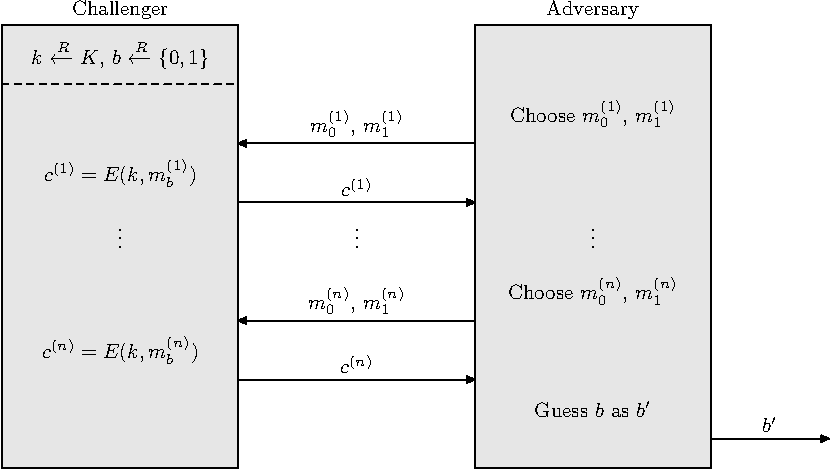
\includegraphics{./figures/game_semsec/game_semsec-1.pdf}
	\caption{Game \ref{game:semsec} depicted.}
	\label{fig:semsecgame}
\end{center}
\end{figure}

\begin{note}   %!% NEW
\label{note:ambigencr}
	The adversary is intentially allowed to provide the same plaintext over and over again. However, it follows that the challenger has to encrypt the same plaintext differently each time, otherwise there would exist a trivially winning adversary.
	
	Indeed, such an adversary would pick three distinct plaintexts $m_0$, $m_1$, $m_2$ and send $(m_0,m_1)$ to the challenger, while she would get back some ciphertext $c_a$. In her second query, the adversary would send $(m_0,m_2)$ to the challenger and receive another ciphertext, say $c_b$. If encryptions of $m_0$ were equal, she could decide with certainty:
	\begin{itemize}
		\item $b' = 0$ if $c_a = c_b$, or
		\item $b' = 1$ otherwise,
	\end{itemize}
	and win the game.
\end{note}

\begin{note}   %!% NEW
\label{note:randomize}
	In order to achieve semantic security of a cipher, the cipher {\em must} encrypt the same plaintext differently each time. This can be achieved using randomization or counters, both approaches are practically used.
\end{note}


\subsubsection{Definition of Semantic Security}

Let us introduce some notion first.

\begin{defn}[Negligible Function]
\label{def:neglfunc}
	Let $\epsilon:\N\rarr\R$. $\epsilon$ is called {\em negligible} if $\forall d\in\N$ $\exists \lambda_0\in\N$ such that $\forall \lambda>\lambda_0$ it holds $\epsilon(\lambda)\leq\frac{1}{\lambda^d}$. In the opposite case, $\epsilon$ is called {\em non-negligible}.
\end{defn}
\nomenclature{$\N$}{Positive integers}
\nomenclature{$\R$}{Real numbers}

\begin{defn}[Overwhelming Function]
\label{def:overwh}
	Let $\epsilon:\N\rarr\R$. $\epsilon$ is called {\em overwhelming} if $1-\epsilon$ is negligible.
\end{defn}

\begin{note}
\label{note:neglconst}
	In practice, {\em negligible} is commonly used with concrete constants as well: $\epsilon<\frac{1}{2^{80}}$ is considered negligible, i.e.\ events with such probability are not considered to occur during our lives. On the other hand, $\epsilon>\frac{1}{2^{30}}$ is considered non-negligible, i.e.\ it is likely to observe an event with such probability.
\end{note}

\begin{defn}[Oracle]
\label{def:oracle}
	Let $F:X\rarr Y$. {\em Oracle evaluating $F$} is a device which, given $x\in X$, evaluates and returns $F(x)$ in unit time; denoted by ${\cal O}_F$.
\end{defn}

\begin{defn}[Oracle with Limited Access]   %!% NEW
\label{def:saoracle}
	Let $F:X\rarr Y$ and $n\in\N$. {\em Oracle with limited access evaluating $F$} is an oracle evaluating $F$, where the number of queries is limited to $n$; denoted by ${\cal O}^{(n)}_F$.
\end{defn}

\begin{defn}[Statistical Test]
\label{def:stattest}
	Let $F:X\rarr Y$. {\em Statistical test} is a (possibly randomized) effective algorithm $A$, which only has an access to an oracle evaluating $F$, and which outputs $0$ or $1$; denoted by $A({\cal O}_F)$.
\end{defn}

\begin{note}
	Statistical test will be also referred to as {\em adversary}.
\end{note}

\begin{defn}[Advantage]
\label{def:advant}
	Let $\cal F$, $\cal G$ be two distinct subsets of the set of all functions from $X$ to $Y$, and let $A$ be an adversary. We define {\em advantage} of adversary $A$ as
	\[
		\Adv(A,{\cal F},{\cal G}) = \left| \Pr\limits_{F\unirand {\cal F}}\Bigl(A({\cal O}_F)=1\Bigr) - \Pr\limits_{G\unirand {\cal G}}\Bigl(A({\cal O}_G)=1\Bigr) \right| .
	\]
\end{defn}

\begin{defn}[Advantage with Limited Access]   %!% NEW
\label{def:saadvant}
	Let $n\in\N$. {\em Advantage with limited access} is defined as advantage, where oracles with access limited to $n$ are used instead; denoted by ${\Adv}^{(n)}$.
\end{defn}

In other words, advantage tells us how likely adversary $A$ is able to distinguish a random function from one set of functions from a random function from another set, based on its input/output behavior only. According to these sets, advantage can be ``customized'' for a specific purpose. Let us define such advantage for an adversary tempting to distinguish which of her plaintexts has been encrypted, i.e.\ tells us how likely she is to win the Game \ref{game:semsec}.

\begin{defn}[Semantic Security Advantage]
\label{def:ssadvant}
	Let $E: K\times M\rarr C$ be an encryption function of a symmetric cipher, ${\cal E}_b = \{E_b:M^2\rarr C \mid E_b(m_0,m_1) = E(k,m_b), k\in K\}$ for $b=0,1$, and $A$ an adversary. We define {\em semantic security advantage} of adversary $A$ as
	\[
		\AdvSS(A,E) = \Adv(A,{\cal E}_0,{\cal E}_1) .
	\]
\end{defn}

Semantic security advantage gives us a reasonable meter for formalization of Game \ref{game:semsec}. Let us use it to define another notion of security, cf.\ Definition \ref{def:perfsec} (Perfectly Secure Cipher).

\begin{defn}[Semantically Secure Cipher]
\label{def:semsec}
	Let $(E,D)$ be a symmetric cipher. Then it is called {\em semantically secure} if, for {\em any} adversary $A$, the semantic security advantage $\AdvSS(A,E)$ is negligible.
\end{defn}

Semantically secure cipher therefore cannot be broken by any probabilistic-polynomial attack with overwhelming probability. On the other hand, it might be broken by an attacker with unlimited computing power -- unlike perfectly secure cipher which cannot be broken by any means; see Note \ref{note:indist}.

The benefit of semantic security over perfect security is that semantic security does not imply any inconvenient consequence analogous to Theorem \ref{thm:kgeqm}, i.e.\ addresses our intention as stated in Note \ref{note:intent}, and practically provides similar security.

Let us now give a nice real-world example, how things can go wrong if semantic security is not complied, even though the design follows common sense.

\begin{example}
\label{ex:crime}
	In 2012, a combination of settings in TLS\footnote{Transport Layer Security, a cryptographic protocol.} allowed researchers to hijack a web session by cracking encrypted cookies \cite{goodin2012crime}. The problem arised when compression was followed by encryption, which actually makes sense. Let us have a look from theoretical point of view.
	
	Remind the condition of Game \ref{game:semsec} -- it requires two plaintexts of equal length. With this assumption, the respective ciphertexts were indistinguishable. However, if the plaintext is compressed first, it can result in differently-sized inputs to the subsequent (semantically secure) cipher! This obviously harms the assumption of inputs of equal length, and may allow the attacker to distinguish the ciphertexts. Note that only very little queries (around six) were needed to attack one byte of an encrypted cookie in the practical attack!
	
	This vulnerability was given a CVE\footnote{Common Vulnerabilities and Exposures, a standard for information security vulnerability names, see \link{http://cve.mitre.org/}.} code CVE-2012-4929 and a human-readable name ``CRIME'' (Compression Ratio Info-leak Made Easy).
\end{example}

\subsubsection{Shannon's Principles}
	
	Before we present how semantic security is practically achieved, let us introduce a principle which is widely followed in cipher design.
	
	\begin{princ}[Shannon]
	\label{pri:shannon}
		As outlined in another Shannon's work \cite{shannon1949communication}, secure ciphers are suggested to employ two basic principles -- {\em confusion} and {\em diffusion}.
		\begin{description}
			\item[Confusion.] The relation between information in plaintext or key and information in respective ciphertext shall be very complex, e.g.\ should not belong to a specific subset of mappings, especially to linear ones.
			\item[Diffusion.] Small piece of information in plaintext or key shall be spread in a long piece of respective ciphertext, e.g.\ one bit of plaintext or key should change a large portion of respective ciphertext.
		\end{description}
	\end{princ}
	
	Semantic security is usually achieved using smaller building blocks, which are required to have certain properties -- they especially make use of confusion and diffusion. The following section describes a building block of one of possible approaches.


% ==============================================================================
% ===   B L O C K   C I P H E R                                              ===
% ==============================================================================

\subsection{Block Cipher}

There are two main approaches how to construct a candidate semantically secure cipher. They make use of
\begin{enumerate}
	\item a {\em stream cipher}, or
	\item a {\em block cipher},
\end{enumerate}
respectively. Stream ciphers achieve semantic security by proper initialization, on the other hand, block ciphers use initialization together with {\em modes of operation}, e.g.\ {\em Cipher Block Chaining} (CBC) or {\em Counter Mode} (CTR). Modes of operation will not be covered in this thesis; only block ciphers and their desired properties will be described, a bunch of definitions follows.

\begin{defn}[Pseudorandom Permutation]
\label{def:prp}
	Let $E: K\times X\rarr Y$. We call $E$ a {\em pseudorandom permutation} (PRP) if there exists an efficient algorithm which evaluates $E$, the function $E(k,\cdot): X\rarr Y$ is a bijection and there exists an efficient algorithm to compute $E^{-1}(k,\cdot)$, for every $k\in K$.
\end{defn}

\begin{note}
	%~ For $X$ and $Y$ being a set of fixed-length strings, e.g.\ $X = Y = \{0,1\}^n$   %?%
	Pseudorandom permutation is usually referred to as {\em block cipher}. Note that the previous definition is in some sense very similar to Definition \ref{def:symcipher} -- it does not introduce any security requirements either.
\end{note}

Pseudorandom permutations will play the main role from now and $k$ will play the role of their key. In order to achieve semantic security of certain constructions using a PRP, we need the PRP to behave indistinguishable from a truly random bijection. Let us demonstrate a possible approach on a game similar to Game \ref{game:semsec}.

\begin{game}
\label{game:prp}
	There are two parties -- a {\em challenger} and an {\em adversary}. Let $E:K\times X\rarr Y$ be a PRP. First, the challenger chooses a random key $k\unirand K$, a random bijection $F:X\rarr Y$ and a random bit $b\unirand\{0,1\}$. Then the adversary sends $x\in X$ of her choice to the challenger. The challenger applies $E(k,\cdot)$ or $F$ if $b=0$ or $1$, respectively, and sends the result back to the adversary. The adversary is allowed to perform several such queries.
	
	The aim of the adversary is to distinguish effectively which $b$ has been chosen by the challenger.
\end{game}

Before we give a formal definition of a secure PRP, we define adversary's advantage in the previous game in a manner analogous to Definition \ref{def:ssadvant}.

\begin{defn}[PRP Advantage]
\label{def:prpadvant}
	Let $E: K\times X\rarr Y$ be a PRP, $\cal B$ the set of all bijections from $X$ to $Y$, and $A$ an adversary. We define {\em PRP advantage} of adversary $A$ as
	\[
		\AdvPRP(A,E) = \Adv\Bigl(A,\bigl\{E(k,\cdot) \bigm| k\in K\bigr\},{\cal B}\Bigr) .
	\]
\end{defn}

PRP advantage tells us how likely adversary $A$ is able to distinguish a PRP with a random key from a truly random bijection based on its input/output behavior only. The definition of secure PRP follows.

\begin{defn}[Secure PRP]
\label{def:secprp}
	Let $E: K\times X\rarr Y$ be a PRP. Then it is called {\em secure PRP} if, for {\em any} adversary $A$, the PRP advantage $\AdvPRP(A,E)$ is negligible.
\end{defn}

In other words, given a random key, PRP is secure if it is computationaly indistinguishable from a truly random bijection. 

An example covering most introduced concepts follows.

\begin{example}
	Let $E:\{0,1\}^{128}\times\{0,1\}^{128}\rarr\{0,1\}^{128}$ be a PRP defined as
	\[
		E(k,x) = \bin\bigl((k)_2 + (x)_2\mod{2^{128}}\bigr)
	\]
	where $\bin(\cdot)$ stands for number's $128$-bit binary representation and $(\cdot)_2$ stands for a number represented by given binary string.
	
	Now let us construct an adversary $A$ as follows: it generates two arbitrary but distinct $x_0,x_1\in\{0,1\}^{128}$, and feeds them to an oracle computing either PRP $E$, or a truly random bijection. The oracle returns $y_0$ and $y_1$, respectively, and the adversary compares values $(y_i)_2 - (x_i)_2 \mod{2^{128}}$ for $i=0,1$ with each other. If these values are equal, $A$ returns $1$, otherwise it returns $0$.
	
	Note that if the oracle computes PRP $E$, then these values are always equal. Otherwise -- i.e.\ the oracle computes a truly random bijection -- the values are distinct with overwhelming probability. Therefore the PRP advantage of such adversary is
	\[
		\AdvPRP(A,E) = \left| \Pr\limits_{k\unirand \{0,1\}^{128}}\Bigl(A\bigl({\cal O}_{E(k,\cdot)}\bigr)=1\Bigr) - \Pr\limits_{F\unirand {\cal B}}\Bigl(A({\cal O}_F)=1\Bigr) \right| = 1 - \epsilon ,
	\]
	where $\cal B$ stands for the set of all bijections on $\{0,1\}^{128}$ and $\epsilon$ is negligible.
	
	It follows that such PRP is totally insecure, since there exists an attacker with overwhelming advantage, but only a negligible advantage is allowed.
\end{example}

\begin{note}   %!% NEW
\label{note:secbyobsc}
	In the previous example, the adversary exploits the knowledge of the block cipher's internal structure -- she knows everything but the key. One could have an idea to hide the structure from the attacker, but this is actually a {\em very} bad idea. Once our construction leaks, we need to deploy a new ciphering algorithm confidentially, but we have no way to do so. Moreover, note that a secure PRP was required to be resistant to {\em all} adversaries, hence hiding your design has absolutely no theoretical support.
	
	We shall rather use a secure publicly known block cipher and only rely on the key. Once our key is compromised, we simply establish a new key. Also note that our key is only to be protected within our device, but the ciphering algorithm would have to be protected globally.
	
	Such approach -- hiding the design of a cipher -- is referred to as {\em security by obscurity} and shall be strictly avoided.
\end{note}

This idea has already been addressed in 1883 by Kerckhoffs \cite{auguste1883cryptographie}. It is usually referred to as {\em Kerckhoffs' Principle} and its six rules follow (originally french, english translation taken from \cite{petitcolas2016kerckhoffs}):
\begin{princ}[Kerckhoffs]
	~
	\begin{enumerate}
		\item The system must be substantially, if not mathematically, undecipherable;
		\item The system must not require secrecy and can be stolen by the enemy without causing trouble;\label{item:kerck}
		\item It must be easy to communicate and retain the key without the aid of written notes, it must also be easy to change or modify the key at the discretion of the correspondents;
		\item The system ought to be compatible with telegraph communication;
		\item The system must be portable, and its use must not require more than one person;
		\item Finally, given the circumstances in which such system is applied, it must be easy to use and must neither stress the mind or require the knowledge of a long series of rules.
	\end{enumerate}
\end{princ}
Hence harming rule \ref{item:kerck} from the previous list leads to security by obscurity as introduced in Note \ref{note:secbyobsc}.


% ==============================================================================
% ===   P R O V A B L E   S E C U R I T Y   P R O O F S                      ===
% ==============================================================================

%~ \subsection{Provable Security Proofs}
\subsection{Output Indistinguishability of a Secure PRP}

Now we know what a secure PRP is (or a secure block cipher) -- it is based on Game \ref{game:prp}, where the aim of the adversary is to distinguish a PRP from a truly random bijection. The obvious question is, what happens if we put a secure PRP into Game \ref{game:semsec}, where the adversary tempts to distinguish which of his two inputs has been processed.

Note that PRP {\em is} a cipher (cf. Definition \ref{def:symcipher} and \ref{def:prp}), so it makes sense. Indeed, given a PRP, there exists an effective algorithm evaluating it and its inverse, and also Equation \ref{eq:correct} holds.

\begin{note}   %!% NEW
\label{note:singleaccess}
	PRP has no ambiguity, hence we will need to either limit the amount of adversary-challenger queries to one, or, equivalently, change the key after each query. If we did not do so, then there would obviously exist a trivially winning adversary as outlined in Note \ref{note:ambigencr}.
\end{note}

Let us modify Game \ref{game:semsec} in a manner described in Note \ref{note:singleaccess} for the purpose of testing PRPs.

\begin{game}
\label{game:semsecprp}
	There are two parties -- a {\em challenger} and an {\em adversary}. Let $E:K\times X\rarr Y$ be a PRP. First, the challenger chooses a random key $k\unirand K$ and a random bit $b\unirand\{0,1\}$. Then the adversary sends two equally long plaintexts $m_0$, $m_1$ of her choice to the challenger. The challenger computes $c = E(k,m_b)$ and sends it back to the adversary. The adversary is limited to one query only.
	
	The aim of the adversary is to distinguish effectively which $b$ has been chosen by the challenger.
\end{game}

Based on the previous game, let us define {\em PRP semantic security advantage} and {\em semantically secure PRP} (cf. Game \ref{game:semsec}, Definition \ref{def:ssadvant} and \ref{def:semsec}). % The difference is basically in the oracle access.

%!% nahradit opravdickejma definicema BEGIN

\begin{defn}[PRP Semantic Security Advantage]
\label{def:prpssadvant}
	Let $E: K\times X\rarr Y$ be a PRP, ${\cal E}_b = \{E_b:X^2\rarr Y \mid E_b(x_0,x_1) = E(k,x_b), k\in K\}$ for $b=0,1$, and $A$ an adversary. We define {\em PRP semantic security advantage} of adversary $A$ as
	\[
		\AdvPRPSS(A,E) = {\Adv}^{(1)}(A,{\cal E}_0,{\cal E}_1) .
	\]
\end{defn}

\begin{defn}[Semantically Secure PRP]
\label{def:semsecprp}
	Let $E: K\times X\rarr Y$ be a PRP. Then it is called {\em semantically secure PRP} if, for {\em any} adversary $A$, the PRP semantic security advantage $\AdvPRPSS(A,E)$ is negligible.
\end{defn}

%!% END

The following theorem provides a connection of Game \ref{game:prp} and \ref{game:semsecprp}. It claims that, given a PRP $E$ winning Game \ref{game:prp}, i.e.\ $E$ is indistinguishable from a truly random bijection, $E$ wins Game \ref{game:semsecprp} as well, i.e.\ no adversary can distinguish encryption of $m_0$ from encryption of $m_1$.

\begin{thm}
\label{thm:semsecprp}
	Let $E: K\times X\rarr Y$ be a secure PRP. Then it is also a semantically secure PRP.
\end{thm}
\begin{proof}
	We show that for every PRP semantic security adversary $A$, there exist PRP security adversaries $B_0$, $B_1$ such that
	\begin{equation}
	\label{eq:aleqbb}
		\AdvPRPSS(A,E) \leq \AdvPRP(B_0,E) + \AdvPRP(B_1,E) .
	\end{equation}
	The claim then easily follows -- if $E$ is a secure PRP, i.e.\ $\AdvPRP(B_0,E) + \AdvPRP(B_1,E)$ is negligible, then also $\AdvPRPSS(A,E)$ is negligible. Hence $E$ is a semantically secure PRP.
	
	Let us first denote $W_b$ the event when adversary $A$ answers $1$ while the true value of the PRP semantic security game is $b$, for $b=0,1$. In this notation, it holds
	\begin{equation}
	\label{eq:prpssae}
		\AdvPRPSS(A,E) = \bigl| \Pr(W_1) - \Pr(W_0) \bigr| .
	\end{equation}
	Let us further denote $R_b$ the same event with only difference -- the PRP semantic security game uses a truly random bijection instead. It holds
	\begin{equation}
	\label{eq:rr0}
		\bigl| \Pr(R_1) - \Pr(R_0) \bigr| = 0 ,
	\end{equation}
	since $b\unirand\{0,1\}$ and both $R_b$ provide a truly random bijection independent from $b$.
	
	Now we construct adversaries $B_0$, $B_1$ distinguishing PRPs from truly random ones while we make use of adversary $A$. Let us construct $B_0$ first. We ask $A$ to provide $m_0$ and $m_1$, then we feed the PRP oracle with $m_0$ obtaining $c$ as a result. Note that either $c=E(k,m_0)$ or $c=F(m_0)$ according to $b$, where $F$ is a truly random bijection. We provide this $c$ to adversary $A$, and output what $A$ outputs. The advantage of adversary $B_0$ is
	\begin{equation}
	\label{eq:prpb0}
		\AdvPRP(B_0,E) = \left| \Pr(W_0) - \Pr(R_0) \right| .
	\end{equation}
	We construct $B_1$ in a similar manner (i.e.\ choosing $m_1$ instead) and get
	\begin{equation}
	\label{eq:prpb1}
		\AdvPRP(B_1,E) = \left| \Pr(W_1) - \Pr(R_1) \right| .
	\end{equation}
	Combining Equations \ref{eq:prpssae}, \ref{eq:rr0}, \ref{eq:prpb0} and \ref{eq:prpb1}, we get
	\begin{align*}
		\AdvPRPSS(A,E) &= \left| \Pr(W_1) - \Pr(W_0) \right| \leq \\
		&\leq \left| \Pr(W_1) - \Pr(R_1) \right| + \left| \Pr(W_0) - \Pr(R_0) \right| = \\
		&= \AdvPRP(B_1,E) + \AdvPRP(B_0,E) ,
	\end{align*}
	which finally proves Equation \ref{eq:aleqbb}, hence the theorem, too
\end{proof}

\begin{note}
	The previous theorem does not work the other way around, i.e.\ a semantically secure PRP does not need to be a secure PRP. Indeed, let $E: K\times X\rarr Y$ be a secure PRP, and let us define $E'(k,x) = E(k,x)\|1$, where $\|$ stands for string concatenation. $E'$ is obviously semantically secure (it remains hard to distinguish encryptions of dinstinct plaintexts), but it can be easily distinguished from a truly random bijection, since it always ends with $1$. The advantage of such adversary would be $\AdvPRP(A,E') = \nicefrac{1}{2}$ which is clearly non-negligible.
\end{note}
\nomenclature{$a \parallel b$}{Concatenation of strings $a$ and $b$}

The previous theorem is especially important for the idea behind its proof which is used in many other proofs related to provable-security. In this proof, we constructed adversaries $B_0$, $B_1$, which internally employed adversary $A$, and then we used advantage of $A$ to estimate advantages of $B_0$ and $B_1$.


% ==============================================================================
% ===   P R O V A B L E   V S   R E A L - W O R L D                          ===
% ==============================================================================

\subsection{Provable vs. Real-World Security}
\label{sec:provable}

Provable security is one aspect, the other is practical construction of a cipher. Note that there is no provably secure block cipher known.

If there were, it would actually imply that $\Pclass \subsetneq \NPclass$ which is an open millenium problem. Indeed, if $\Pclass = \NPclass$ and $E$ were a PRP, then the adversary could, given certain (polynomial) amount of plaintext-ciphertext pairs $(m_i,c_i)$, non-deterministically find a key $k$, such that $c_i = E(k,m_i)$ for all $i$. Then she would simply answer ``truly random'' if no such $k$ were found, otherwise she says ``pseudorandom''. Here, the ``truly random'' answer is answered with certainty, while the ``pseudorandom'' answer is just a conjecture, but it has sufficiently large probability.
\nomenclature{$\Pclass$}{Deterministic polynomial complexity class i.e.\ the set of decision problems which can be solved by a deterministic Turing machine in polynomial time}
\nomenclature{$\NPclass$}{Non-deterministic polynomial complexity class i.e.\ the set of decision problems which can be solved by a non-deterministic Turing machine in polynomial time}

Instead, real-world block ciphers are {\em beleived} to be secure based on a simple fact: no known attack is far better than exhaustive search. One such block cipher is called {\em Advanced Encryption Standard} (AES) and will be of top interest in this thesis. AES will be described in detail in Section \ref{sec:aes}.


% ==============================================================================
% ===   F R O M   B L A C K - B O X   T O   W H I T E - B O X                ===
% ==============================================================================

\subsection{From Black-Box to White-Box Attack Context}
\label{sec:bbtowb}

The other central topic of this thesis is {\em white-box attack context}. In order to explain what it is, let us begin with {\em black-box attack context}.

\subsubsection{Black-Box}

First of all, as stated in Note \ref{note:threat}, we need to address attacker's abilities -- the threat model. In the black-box model, the attacker is granted an access to an oracle evaluating given encryption algorithm $E$ with a random secret key $k$, while the (primary) goal of the attacker is to recover the key. The attacker has absolutely no information but inputs and respective outputs, she cannot observe any internal routines of the encryption procedure, hence black-box.

\begin{note}
	There could be many other goals than just key recovery, e.g.\ guessing the ciphertext in advance, or decrypting certain/given ciphertext with non-negligible probability and so on. Actually whatever one can imagine, which would be in principle possible with a PRP, but not with a truly random bijection.
\end{note}

Classical ciphers are designed under the assumption of black-box attack context, therefore their implementation must be extremely careful. The attacker could for example measure the time of encryption and exploit this information, which was not considered during the design of the cipher.

\subsubsection{Gray-Box}

Gray-box attack context is closer to reality, since we do not encrypt using oracles, but rather using some physical device, which runs a specific implementation of given cipher. In the gray-box model, cipher is thus supposed to be implemented and run, while the attacker can observe some information related to cipher's intermediate results as well.

Such information leaks can be modelled as a set of distributions conditioned by intermediate results and are referred to as {\em leakage model}. There is an area of theoretical cryptography studying leakages -- {\em Leakage Resilient Cryptography}. A practical attack exploiting such leaks will be described in Chapter \ref{chap:attack} in Section \ref{sec:side}.   %?% LRC introduced by?

\subsubsection{White-Box}

Finally, there is the most extreme case where the attacker has full control over the execution environment -- the {\em white-box attack context} (WBAC). Full control means that the attacker can step the algorithm and directly observe and alter intermediate results in the memory, or even skip, alter and insert instructions. Clearly, the key cannot be kept in its original form, it must be somehow hidden, but still usable for encryption.
